\ifdefined\ingles	
	The boom of the current graph databases gives us important possibilities when it comes to modeling a domain for which the relational databases have no direct application.
	
	The possibility of including in the designed schema information of various types, without penalizing for them the search capabilities or the representativeness of the information, is one of the most favorable characteristics of the graph-based model, which makes it especially recommendable in environments where there is no established scheme or is not stable or suffers from frequent variations. Examples of this are design prototypes, databases for concept testing and storage for data mining\cite{robinson2015graph}.
	
	In terms of expressiveness, the graph databases reduce the impedance difference between the analysis model and the final implementation, a problem that has plagued the various database models for many years.
	
	\subsection {Representation factors}
	
	In order to have relevant information of the chosen domain and be able to detect patterns, it is necessary to have a graph base that represents the information of the star clusters with the greatest possible accuracy.
	
	Currently, at least four fundamental factors must be taken into account when designing a system of knowledge representation in any given domain\cite{van2008handbook}:
	
	\begin{itemize}
		\item \textbf{Representational Adecuation:} Ability to represent all kinds of knowledge that are necessary in the domain.
		\item \textbf{Inferential Adecuation:} Ability to manipulate representation structures in such a way that they generate new structures that correspond to new knowledge inferred from the previous ones.
		\item \textbf{Inferential Efficiency:} Ability of the system to incorporate additional information to the representation structure, called meta-knowledge, which can be used to focus the attention of the inference mechanisms in order to optimize the computations.
		\item \textbf {Acquisition Efficiency:} Ability to easily incorporate new information. Ideally the system itself should be able to control the acquisition of new information and its subsequent representation.
	\end{itemize}
	
	These factors were taken into account during the process of designing the structures of the database, in such a way that the results can be maximized while computing operations are kept efficient.
	
	\subsection{The model of tagged graphs}
	
	The approach proposed in the present work is based on the tagged graph model, existing in a multitude of graph database products, both commercial and Open Source.
	
	A \emph{tagged properties graph} is composed of nodes, relationships, properties and labels, as can be seen in Figure \ref{fig:property-graph-model-eng}.
	
	\begin{figure}[h]
		\centering
		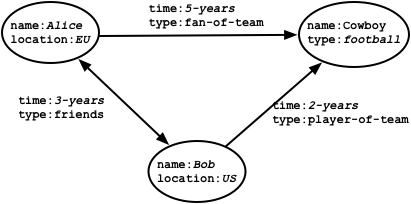
\includegraphics[scale=0.5]{./images/property-graph-model}
		\caption{Property Graph Model}
		\label{fig:property-graph-model-eng}
	\end{figure}

	\begin{itemize}
		\item The \textbf{nodes} contain \textbf{properties}. You can think of nodes as documents that group together a set of properties that define the characteristics of the document to which they belong.
		\item The \textbf{nodes} can be marked with one or more \textbf {labels}. Labels group nodes by similar characteristics or indicate the roles each plays in the data model.
		\item The \textbf{links} connect nodes to each other and define the structure of a graph. A link has an direction, a source node and a destination node.
		\item Like nodes, links can also have properties that add semantic value to the relationship.
		\item In all cases, the properties and their values can be used to restrict the results of searches performed in a graph.
	\end{itemize}

	Based on the theoretical model of tagged graphs discussed above, an implementation model was designed that will provide support to the data on which the recognition algorithms will act.

	The central element to be considered in the implementation model are the \textbf{nodes}. The nodes, in this area, model individual readings obtained by the observation instrument. Each node becomes equivalent, with this approach, to a record of the information exchange files. This process will be detailed in the section \ref{sec:sources-preprocessing}.
	
	A unique identifier will be generated for each node to simplify the queries and subsequent recovery of the information associated with them. There are some properties inherent to each of the observations that will be stored in the corresponding nodes, such as the coordinates of that observation, the section of the sky that is being surveyed and the settings of the observation instrument. All these characteristics are necessary to reconstruct the original observation conditions from the data.
	
	The \textbf {labels}, once the general data of each node is imported, will play a fundamental role since they are responsible for the storage of all the additional information that will be used in the searches.
	
	Among the possible values to be stored are the various readings taken by the instruments and optical processors of the telescopes from which the information is obtained, including readings in the optical spectrum as well as in the infrared or ultraviolet (identified with certain particular wavelengths), labels relating to brightness, rotation speed, nomenclature, etc. will also be incorporated.
	
	In the graph model the relations between the nodes are of crucial importance for the paths and are fundamental for the detection of patterns. But in the field under study it must be recognized that there is no single characteristic that links two stars and their associated readings.
	
	There are many parameters that can indicate relations, such as the distance between the stars, the luminosity, the size, the different spectral readings, their rotation period, etc. As it is impracticable to establish relationships for all possible combinations of characteristics, the implementation will allow generating those relationships on demand.
	
	That is, as a preliminary step to the analysis and detection of patterns, the user must indicate which feature or combination of them he wants to use to generate the relationships between the stars. Then the indicated relationships will be generated and the analysis will be made based on the resulting graph with the structure determined according to the characteristics indicated by the user.
	
	This approach has been used in a timely manner in the papers published by Coutinho et. al 2016 \cite{coutinho2016network}, an example of which is presented in Figure \ref{fig:galaxies-as-graph-eng}.
	
	\begin{figure}[h]
		\centering
		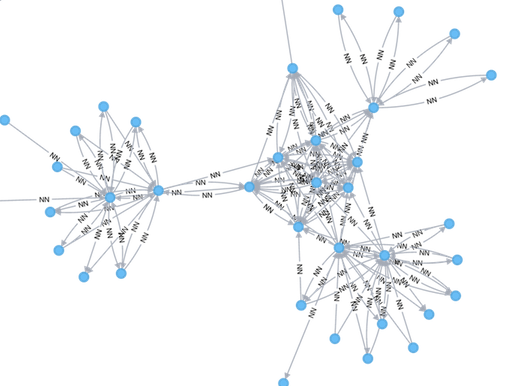
\includegraphics[width=0.7\linewidth]{./images/galaxies-graph-visualization-small}
		\caption{Galaxies as labeled graph. Coutinho et. al}
		\label{fig:galaxies-as-graph-eng}
	\end{figure}
	
	\subsection{Sources and pre-processing of data} \label{sec:sources-preprocessing}
	
	The aforementioned astronomical survey projects have large repositories of publicly accessible information, which are going to be used as sources of information to load the analysis database.
	
	The \emph{de facto} standard for the exchange of astronomical information is based on the FITS file format (Flexible Image Transport System\cite{hanisch2001definition}) which will be used as a basis for all data import routines.
	
	ONgDB, the database used in this work, has the possibility of importing data files in a massive way, which is very necessary because each one of the source files generally have volumes of approximately half a million records. For this, it uses comma separated files with a particular format.
	
	It is necessary to pre-process the information so that it is in an adequate format for its massive import into the database. To this end, a Python language development is proposed, which provides the AstroPy \cite{robitaille2013astropy} libraries that are suitable for the reading and parsing of FITS files and allows the CSV files to be managed with ease. The complete procedure is described in Figure \ref{fig:import-data-eng}.
	
	\begin{figure}[h]
		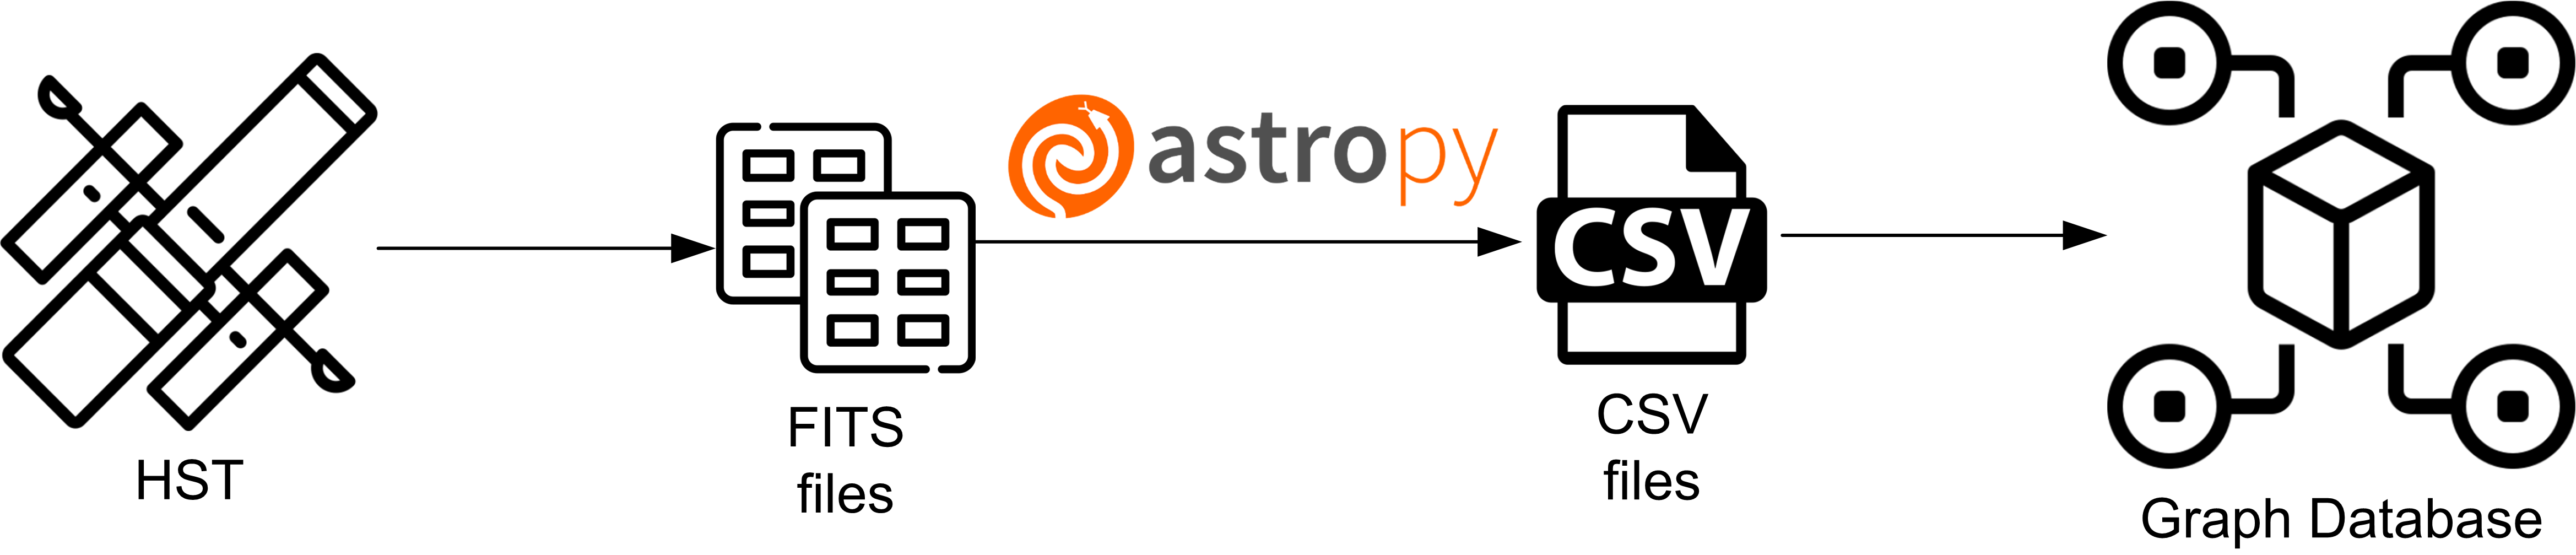
\includegraphics[width=\linewidth]{./images/importacion-datos}
		\caption{Data pre-processing and import flow}
		\label{fig:import-data-eng}
	\end{figure}

	\subsection{Selected storage}
	
	For the implementation of the data model we opted for the use of ONgDB (\url{https://www.graphfoundation.org/projects/ongdb/}), a completely Open Source alternative to Neo4J (\url{https://neo4j.com/}), which is perhaps the most widespread commercial graph database.
	
	We chose this product because it has some very valuable characteristics for the project:
	
	\begin{itemize}
		\item Natively represents the characteristics of the labeled graph model mentioned above
		\item Based on a commercial product of proven quality and updated technology
		\item It has a non-restrictive license that allows it to be used freely and free of charge in educational institutions and as part of research projects
		\item It has no restrictions regarding advanced features such as
		\begin{itemize}
			\item ACID Transactions
			\item Replication
			\item Monitoring
		\end{itemize}
	\end{itemize}
\else
	El auge de las actuales bases de datos de grafos nos brinda posibilidades importantes a la hora de modelar un dominio para el cual las bases de datos relacionales no tienen aplicación directa.
	
	La posibilidad de incluir en el esquema diseñado, información de tipos variados, sin penalizar por ellos las capacidades de búsqueda o la representatividad de la información es una de las características más favorables del modelo basado en grafos, lo que la hace especialmente recomendable en entornos en donde no se cuenta con un esquema establecido o no es estable o sufre fercuentes variaciones, ejemplos de esto son prototipos de diseño, bases de datos para la prueba de conceptos y almacenamientos para minería de datos\cite{robinson2015graph}.
	
	En términos de expresividad las bases de datos reducen la diferencia de impedancia entre el modelo de análisis y la implementación final, un problema que ha acosado a los diversos modelos de bases de datos desde hace muchos años.
	
	\subsection{Factores de representación}
	
	Para tener información relevante del dominio elegido y poder detectar patrones, se necesita contar con una base de grafos que represente la información de los cumulos estelares con la mayor exactitud posible.
	
	Actualmente se deben tener en cuenta al menos cuatro factores fundamentales a la hora de diseñar un sistema de representación del conocimiento en cualquier dominio dado\cite{van2008handbook}:
	
	\begin{itemize}
		\item \textbf{Adecuación Representacional:} Habilidad para representar todas las clases de conocimiento que son necesarias en el dominio.
		\item \textbf{Adecuación Inferencial:} Habilidad de manipular estructuras de representación de tal manera que devengan o generen nuevas estructuras que correspondan a nuevos conocimientos inferidos de los anteriores.
		\item \textbf{Eficiencia Inferencial:} Capacidad del sistema para incorporar información adicional a la estructura de representación, llamada metaconocimiento, que puede emplearse para focalizar la atención de los mecanismos de inferencia con el fin de optimizar los cómputos.
		\item \textbf{Eficiencia en la Adquisición:} Capacidad de incorporar fácilmente nueva información. Idealmente el sistema por sí mismo deberá ser capaz de controlar la adquisición de nueva información y su posterior representación.
	\end{itemize}
	
	Estos factores se tuvieron en cuenta durante el proceso de diseño de las estructuras de la base de datos, de manera tal que se puedan maximizar los resultados a la vez que se mantienen eficientes las operaciones de cómputo.
	
	\subsection{El modelo de grafos etiquetados}
	
	El enfoque propuesto en el presente trabajo se basa en el modelo de grafos etiquetados, existente en multitud de productos de base de datos de grafos, tanto comerciales como Open Source.
	
	Un \emph{grafo de propiedades etiquetadas} esta compuesto de nodos, relaciones, propiedades y etiquetas, tal como se puede apreciar en la Figura \ref{fig:property-graph-model}.
	
	\begin{figure}[h]
		\centering
		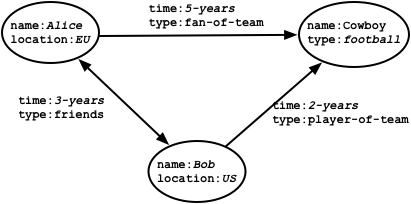
\includegraphics[scale=0.5]{./images/property-graph-model}
		\ifdefined\ingles
			\caption{Property Graph Model}
		\else
			\caption{Modelo de Grafo Etiquetado}
		\fi
		\label{fig:property-graph-model}
	\end{figure}
	
	
	\begin{itemize}
		\item Los \textbf{nodos} contienen \textbf{propiedades}. Se puede pensar en los nodos como documentos que agrupan un conjunto de propiedades que definen las características del documento al que pertenecen. 
		\item Los \textbf{nodos} pueden ser marcados con una o más \textbf{etiquetas}. Las etiquetas agrupan nodos por características similares o indican los roles que cada uno juega en el modelo de datos.
		\item Las \textbf{relaciones} conectan nodos entre si y definen la estructura de un grafo. Una relación tiene una dirección, un nodo de origen y un nodo de destino.
		\item Como los nodos las relaciones también pueden tener propiedades que le agregan valor semántico a la relación.
		\item En todos los casos, las propiedades y sus valores pueden utilizarse para restringir los resultados de las búsquedas realizadas en un grafo.
	\end{itemize}
	
	En base al modelo teórico de grafos etiquetados expuesto anteriormente se diseñó un modelo de implementación que brindará soporte a los datos sobre los que actuarán los algoritmos de reconocimiento.
	
	El elemento central a considerar en el modelo de implementación son los \textbf{nodos}. Los nodos, en este ámbito modelan lecturas puntuales obtenidas por el instrumento de observación. Cada nodo se hace equivalente, con este enfoque, a un registro de los archivos de intercambio de información. Este proceso se detallará en la sección \ref{sec:fuentes-preprocesamiento}.
	
	Se generará un identificador único para cada nodo para simplificar las consultas y posterior recuperación de la información asociada a los mismos. Existen algunas propiedades inherentes a cada una de las observaciones que serán almacenadas en los nodos correspondientes, como por ejemplo las coordenadas de dicha observación, la sección del cielo que se está relevando y los ajustes del instrumento de observación. Todas estas características son necesarias para reconstruir las condiciones originales de observación a partir de los datos.
	
	Las \textbf{etiquetas}, una vez importados los datos generales de cada nodo, pasarán a cumplir un rol fundamental ya que son las responsables del almacenamiento de toda la información adicional que se utilizará en las búsquedas.
	
	Dentro de los posibles valores a almacenar se encuentran las diversas lecturas tomadas por los instrumentos y procesadores ópticos de los telescopios de dónde se obtiene la información, incluyendo lecturas en el espectro óptico así como en el infrarrojo o ultravioleta (identificados con ciertas longitudes de onda particulares), también se incorporarán etiquetas relativas a luminosidad, velocidad de rotación, nomenclatura, etc.
	
	En el modelo de grafos las relaciones entre los nodos son de crucial importancia para los caminos y son fundamentales para la detección de patrones. Pero en el ámbito bajo estudio hay que reconocer que no existe una única característica que relaciones dos estrellas y sus lecturas asociadas.
	
	Existen multitud de parámetros que pueden indicar relaciones, tales como la distancia entre las estrellas, la luminosidad, el tamaño, las diferentes lecturas espectrales, su período de rotación, etc. Como es impracticable establecer relaciones para todas las posibles combinaciones de características, la implementación permitirá generar dichas relaciones a demanda.
	
	Es decir, como paso previo al análisis y detección de patrones, el usuario deberá indicar qué característica o combinación de ellas quiere utilizar para generar las relaciones entre las estrellas. Acto seguido se generarán las relaciones indicadas y el análisis se realizará en base a el grafo resultante con la estructura determinada de acuerdo a las características indicadas por el usuario.
	
	Dicho enfoque se ha utilizado oportunamente en los trabajos publicados por Coutinho et. al 2016\cite{coutinho2016network}, un ejemplo de lo cual se presenta en la Figura \ref{fig:galaxies-as-graph}.
	
	\begin{figure}[h]
		\centering
		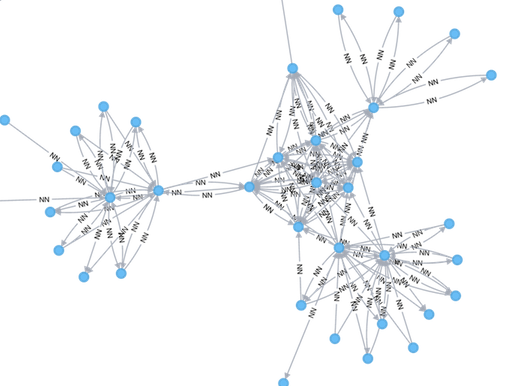
\includegraphics[width=0.7\linewidth]{./images/galaxies-graph-visualization-small}
		\ifdefined\ingles
			\caption{Galaxies as labeled graph. Coutinho et. al}
		\else
			\caption{Galaxias representadas como grafo etiquetado. Coutinho et. al}
		\fi
		\label{fig:galaxies-as-graph}
	\end{figure}
	
	
	\subsection{Fuentes y pre-procesamiento de los datos}\label{sec:fuentes-preprocesamiento}
	
	Los mencionados proyectos de survey astronómicos cuentan con grandes repositorios de información accesible de forma pública, los cuales van a ser utilizados como fuentes de información para cargar la base de datos de análisis.
	
	El estandar de facto para el intercambio de información astronómica se basa en el formato de archivos FITS (Flexible Image Transport System\cite{hanisch2001definition}) el cual será utilizado como base para todas las rutinas de importación de datos.
	
	ONgDB cuenta con la posibilidad de importar archivos de datos de forma masiva, lo cual es muy necesario debido a que los archivos fuente generalmente cuentan con volúmenes de aproximadamente medio millón de registros. Para ello utiliza archivos separados por comas con un formato particular 
	
	Es necesario realizar un procesamiento previo de la información para que la misma se encuentre en un formato adecuado para su importación masiva en la base de datos. Para ello se propone un desarrollo en lenguaje Python, el cual provee las librerías AstroPy\cite{robitaille2013astropy} que son adecuadas para la tarea de lectura y parseo de los archivos FITS y permite gestionar con cierta facilidad los archivos CSV de destino. El procedimiento completo está descripto en la Figura \ref{fig:importacion-datos}.
	
	\begin{figure}[h]
		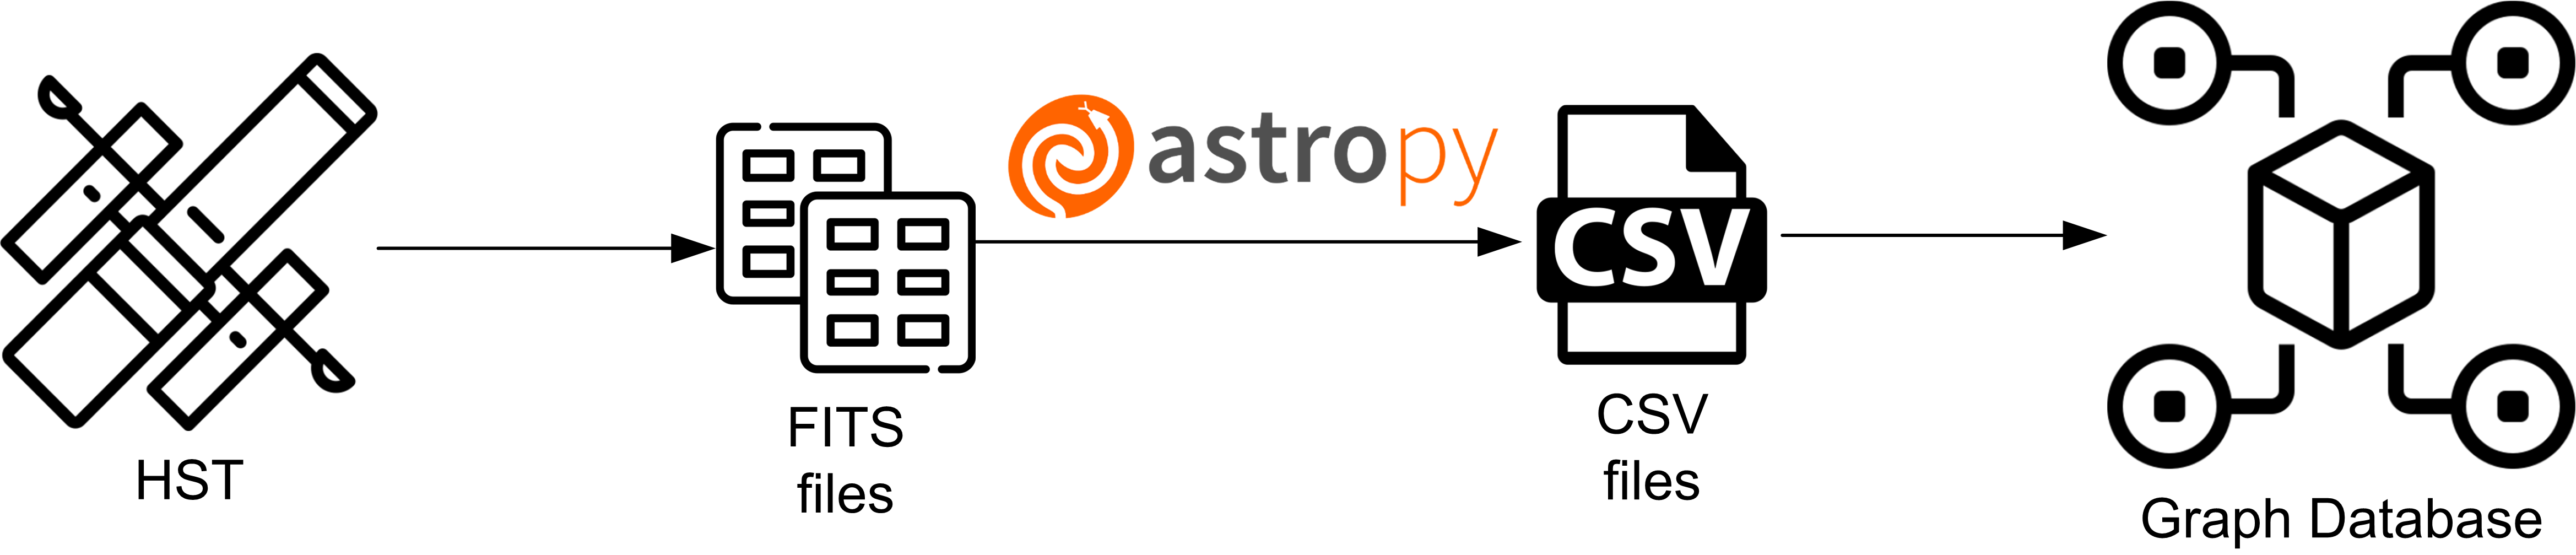
\includegraphics[width=\linewidth]{./images/importacion-datos}
		\ifdefined\ingles
		\caption{Data pre-processing and import flow}
		\else
		\caption{Pre-procesamiento e importación de datos}
		\fi
		\label{fig:importacion-datos}
	\end{figure}
	
	\subsection{El almacenamiento seleccionado}
	
	Para la implementación del modelo de datos se optó por la utilización de ONgDB (\url{https://www.graphfoundation.org/projects/ongdb/}), una alternativa completamente Open Source a Neo4J (\url{https://neo4j.com/}), la que quizá sea la base de datos de grafos comercial más difundida.
	
	Se optó por este producto debido a que reúne algunas características muy valiosas para el proyecto:
	
	\begin{itemize}
		\item Representa de forma nativa las características del modelo de grafo etiquetado mencionado anteriormente
		\item Se basa en un producto comercial de probada calidad y tecnología actualizada
		\item Dispone de una licencia no restrictiva que permite utilizarlo de manera libre y gratuita en instituciones educativas y como parte de proyectos de investigación
		\item No tiene restricciones en cuanto a características avanzadas tales como
		\begin{itemize}
			\item Transacciones ACID
			\item Replicación
			\item Monitoreo
		\end{itemize}
	\end{itemize}
	
	%\subsection{El diseño físico de la base de datos}
	%
	%ESTA SECCION NO SE SI TIENE MUCHO SENTIDO, NO DICE MUCHO, YO LA PUSE EN FUTURO PORQUE NO DICE NADA DE COMO ESTA DISEÑADA LA BASE DE DATOS
	%SI LA DEJAS YO LA PONDRÍA ANTES DE LA SECCION DE ALMACENAMIENTO SELECCIONADO
	%
	%El diseño físico de la base de datos de grafos subyacente para el análisis y detección de patrones tiene un impacto directo y decisivo en el tipo y variedad de los algoritmos que se pueden utilizar y en el rendimiento general del sistema. 
	%
	%Este diseño debería balancear dos elementos importantes, que muchas veces se contraponen. Por una parte el diseño debería ser lo suficientemente genérico y flexible como para permitir representar las lecturas astronómicas actualmente disponibles, como permitir la incorporación futura de nuevos valores, adecuar los formatos de archivos de importación o incluir metadatos necesarios para el análisis.
	%
	%Por otra parte las estructuras deberían permitir la utilización de diversos algoritmos, establecidos y probados, de una forma eficiente, así como debería dar la posibilidad de desarrollar, probar e implementar algoritmos desarrollados para los usos específicos mencionados en el presente trabajo.
	%
	%Estas dos necesidades contrapuestas obligan a plantear algunas soluciones de compromiso y a utilizar todos los mecanismos específicos presentes en el motor de base de datos elegido (ONgDB) para mantener un rendimiento aceptable sin sacrificar flexibilidad.
\fi	
